Our human beings can learn new things progressively in time. At a very young age, we can distinguish thousands of different objects and this ability can increasingly develop as we grow up. Moreover, we actually don't treat a new concept in isolation, but try to connect the new concept to the knowledge we already learned, which is referred to as transfer learning. For example, we recognize the animal zebra by referring it to the normal horse with distinctive black and white striped coats. Given a task of the target learning problem, transfer learning works on the scenario that knowledge learned from one or several prior (source) tasks can help the target learning task. 
Based on this, how to utilize the knowledge from multiple sources leads to the research of Multiple Source Transfer
Learning (MSTL). Transferring the knowledge from multiple priors can make the learning procedure extremely efficient by mining the recurrent patterns as well as inferring inductively on the target task \cite{tommasi2014learning}. Taking advantage of this, the first implementation proposed by \cite{fei2006one} using Bayesian approach shows that even with a single example, transfer learning can still get impressive results. Some methods using discriminative approach are proposed in recent years \cite{tommasi2014learning} \cite{kuzborskij2013n} \cite{jie2011multiclass}. Previous study shows that the more prior knowledge the system acquired, the easier a new concept can be learned \cite{Thrun96islearning}.

However, transferring knowledge can consistently boost the learning performance (positive transfer) is based on the fact that the learning procedure can benefit from sufficient related prior knowledge. In some extreme situation, where the source domain and target one are not related, brutal-force transferring the knowledge between them could even degrade the performance of the classifier for target domain. This is often referred to as negative transfer (see Figure \ref{fig:neg}). How to avoid negative transfer is still an open question in transfer learning \cite{Lu201514}. Specifically, how to the measure the transferability of different prior knowledge and obtain a comprehensive and accurate measurement to prevent negative transfer should be studied profoundly. Our work focus on a scenario that transfers the knowledge from multiple sources and we can only access to the model of the source task rather than the data itself. This indicates that the prior knowledge could be incorrect and negative transfer may happen. This scenario can be a very interesting and practical setting in real life, especially for the image recognition task. For certain image database, we can only access to its pre-trained feature representations (like PHOG or color histogram) rather than the images due to the copyright reason or computational prohibition. Meanwhile, the detail of extracting these is not clear as well. Taking PHOG for example, different angle leads to different feature representation and eventually leads to different prior knowledge for classifiers. Without knowing the utility of the prior knowledge, transfer learning may suffer from negative transfer. To maximum the utility of the prior knowledge, the algorithm should be able to set different weight for different prior knowledge according to their transferability instead of aggressively ignoring or utilizing all of them.

On the other hand, when transferring the knowledge from multiple sources, our human beings are able to distinguish their relationships to the target task by trial-and-error learning and make the decision by balancing the weights between the prior knowledge and empirical knowledge of the specific task. For example, a student is asked to pick some pictures of the horse and told what a horse looks like (prior knowledge). After picking some pictures according to the prior knowledge and examined by certain oracle, the student is able to deduce whether the prior knowledge is correct or not (trial-and-error). If the prior knowledge is incorrect (unrelated prior knowledge), at the beginning, the student would make some mistakes. Then the student will change the strategy to rely more on his/her own knowledge learned from previous pictures over the prior knowledge (increase the weight of empirical knowledge). 
Inspired by this, we proposed \hl{our method} that performs with a similar manner. 
We use Least Square Support Vector Machine (LS-SVM) \cite{suykens1999least}, which is adopted by previous works \cite{tommasi2014learning} \cite{kuzborskij2013n}, as our basic model. The decision of each binary LS-SVM is the linear combination of the prior knowledge and empirical knowledge controlled by some transfer parameters. To measure the transferability of each prior knowledge, we estimate our transfer parameters using closed-form leave-one-out (LOO) error. Previous works theoretically suggest that closed-from LOO error can be an efficient way for parameter estimation with a small training set \cite{kuzborskij2013stability} \cite{cawley2006leave}. Then these transfer parameters are optimized by solving a strongly convex problem that can balance the weight between the prior knowledge and empirical knowledge from target task. 

In this paper, we also provide the theoretical proof that the transfer parameters estimate by our algorithm can prevent negative transfer. Extensive empirical experiments show that other transfer learning baselines suffer from negative transfer while our method can autonomously ignore the unrelated prior knowledge to prevent negative transfer. Then, we also show that when the prior knowledge is highly related to the target task, our method can outperform the transfer learning baselines as well.

The rest of this paper is organized as follow:
  
\begin{figure}
\centering
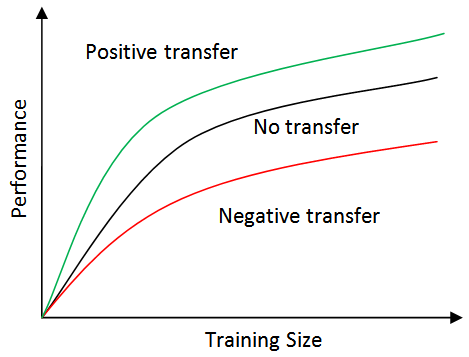
\includegraphics[scale=.6]{fig/negative.png}
\caption{Positive transfer VS Negative transfer. Relying on unrelated priors could lead to negative transfer.}\label{fig:neg}
\end{figure}

%\begin{figure}
%\centering
%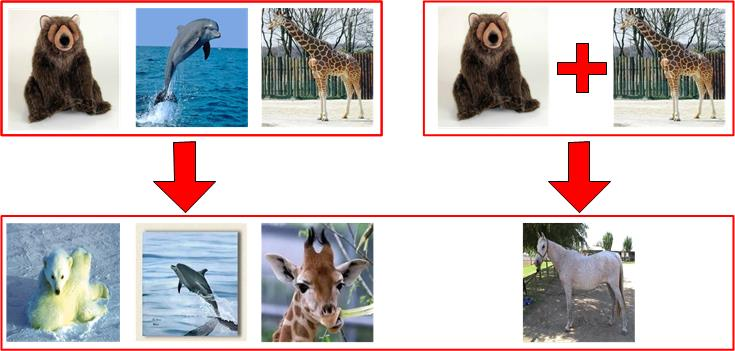
\includegraphics[scale=.4]{fig/transfer.jpg}
%\caption{}\label{fig:combine}
%\end{figure}